\documentclass[a4paper,12pt]{article}
\usepackage[latin1]{inputenc}
\usepackage[spanish]{babel}
\usepackage{bm}
\usepackage{graphicx}
\usepackage{amsmath}
\setlength{\textheight}{235mm}
\setlength{\textwidth}{168mm}
\setlength{\oddsidemargin}{0pt}
\pagestyle{empty}
\begin{document}
\mbox{}\vspace*{-45mm}

{\centering
{\small\sc Escuela T�cnica Superior de Ingenieros de Caminos, Canales y
Puertos (Madrid)}\\*[4mm]
{\Large\bf M�todo de los Elementos Finitos (Curso 19-20)}\\*[4mm]
Ejercicio 1: Estructuras de barras articuladas \\*[4mm]
}

\vspace{3mm}

%%%%%
\noindent

Se considera la estructura de la figura formada por barras articuladas de
acero, cuyo m�dulo el�stico es $E=2.0  \cdot 10^5$ MPa. La secci�n transversal
de cada barra es circular, de di�metro $\phi=25\, \textrm{mm}$. Las dimensiones
y las condiciones de sustentaci�n de la estructura, as� como las cargas
aplicadas, se indican en la figura.

Hacer un modelo de elementos finitos que permita conocer la respuesta mec�nica
de la estructura, y contestar a las preguntas de la hoja adjunta.

\begin{center}
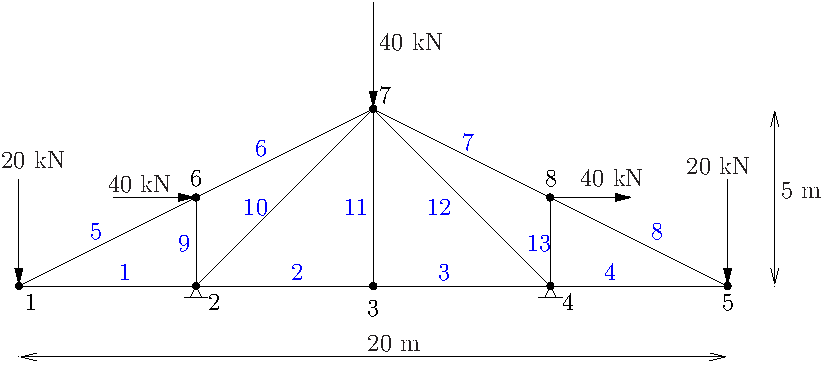
\includegraphics[width=0.75\textwidth]{ej1}
\end{center}
\end{document}
